\documentclass[conference,a4paper]{IEEEtran}
% IEEE conference template (Overleaf "IEEE Conference Template"); a4paper because
% EmergIN 2027's own template is A4. Generated by docs/paper/build/build_paper.py --latex.
\IEEEoverridecommandlockouts
\usepackage{cite}
\usepackage{amsmath,amssymb,amsfonts}
\usepackage{algorithmic}
\usepackage{graphicx}
\usepackage{textcomp}
\usepackage{xcolor}
\usepackage{array}
\usepackage{float}
\usepackage{url}
\usepackage{microtype}   % fewer stretched inter-word spaces in justified columns
\usepackage{flushend}    % balances the two columns on the last page
\def\BibTeX{{\rm B\kern-.05em{\sc i\kern-.025em b}\kern-.08em
    T\kern-.1667em\lower.7ex\hbox{E}\kern-.125emX}}
% tables and figures sit at the top or bottom of a column ([!t]/[!b]), after the text that
% cites them, as the IEEE template asks, so no column ends early; ragged bottoms keep LaTeX
% from stretching the space between paragraphs
\raggedbottom
\begin{document}
\makeatletter
\newcommand{\linebreakand}{\end{@IEEEauthorhalign}\hfill\mbox{}\par\mbox{}\hfill\begin{@IEEEauthorhalign}}
\makeatother
\title{Policy-Guarded Recovery of Known and Unknown Microservice Faults with a Local Large Language Model}

\author{\IEEEauthorblockN{Muhammad Shayaan Ali}
\IEEEauthorblockA{\textit{Dept. of Computer Science and Engineering} \\ \textit{Sharda University} \\ Greater Noida, India \\ {2023433557.muhammad@ug.sharda.ac.in}}
\and
\IEEEauthorblockN{Riddhima Sharma}
\IEEEauthorblockA{\textit{Dept. of Computer Science and Engineering} \\ \textit{Sharda University} \\ Greater Noida, India \\ {2023567320.riddhima@ug.sharda.ac.in}}
\linebreakand
\IEEEauthorblockN{Shruti Tyagi}
\IEEEauthorblockA{\textit{Dept. of Computer Science and Engineering} \\ \textit{Sharda University} \\ Greater Noida, India \\ {2023566902.shruti@ug.sharda.ac.in}}
\and
\IEEEauthorblockN{Aliza Rana}
\IEEEauthorblockA{\textit{Dept. of Computer Science and Engineering} \\ \textit{Sharda University} \\ Greater Noida, India \\ {aliza.rana@sharda.ac.in}}}

\maketitle

\begin{abstract}
Large language models (LLMs) can interpret monitoring data and suggest corrective actions for failing services, but executing these actions on live systems carries risks: a plan may reference the wrong service, include an invented action, or be malformed. This work describes a closed-loop incident response system for microservices in which an anomaly detector and alerting rules identify faults, a locally hosted LLM or rule-based runbooks suggest actions, and a deterministic policy validator alone determines which actions may run. Every executed fix is checked, and an incident that persists is re-analyzed until three attempts have failed and is then escalated. We compare the runbooks, the LLM and the full system over 890 fault-injection runs spanning 18 scenarios on a three-service containerized application, partitioned into faults for which a runbook had been written and faults for which none had, and we test the validator with 29 adversarial plans. No unsafe action was executed in any run or adversarial case. On known faults, runbooks were preferable: the LLM identified the same root causes but chose a less suitable fix in 7.8 percent of runs and added about 29 seconds to recovery. On four unknown faults, the full system resolved 45 percent of runs versus 25 percent for the runbooks: the detector identified faults below the alerting thresholds and the LLM chose a fix where no rule applied, while with the LLM disabled the same detections could only be escalated. Faults that every variant misdiagnosed were escalated after a bounded number of attempts. Our results suggest runbooks for known faults, the LLM where they end, and one guard for both.
\end{abstract}

\begin{IEEEkeywords}
incident response, large language models, AIOps, automated remediation, safety, microservices
\end{IEEEkeywords}

\section{Introduction}

Modern web apps are highly modular systems composed of multiple microservices, and fault propagates along the call chain. If a database slows down, a service calling it will have high latency, and front-end will generate failures, thus, the fired alert will be not the cause of the problem. Incidents continue to be managed by the on-call engineer who will receive an alert, check dashboards, consult a written runbook and apply a fix -- typically it's a service restart or a rollback operation \cite{b1}. Detection is highly mature and fixes are usually scripted, yet the step in between remains manual and time-consuming -- figuring out what went wrong and applying the correct and safe fix.

AIOps (artificial intelligence for IT operations) uses machine learning to find anomalies and group related alerts \cite{b2}, and recent research shows that LLMs can propose root causes and remediation steps for cloud incidents \cite{b3,b4}. Open-source assistants such as k8sgpt \cite{b5} and HolmesGPT \cite{b6} provide natural-language explanations of problems in a cluster. For the most part, these tools offer recommendations; when they are allowed to take actions, their safety depends on the output being correct. An LLM can make up the name of a non-existent service, invent an action, give a confidence that is not a number, or repeat a fix that has already failed, and executing such output directly can turn a small incident into an outage.

This paper explores whether the step of remediation can be delegated to the LLM in case it's treated as an untrusted advisor within a closed control loop -- the LLM provides a plan, policy validator who trusts neither the problem nor the plan checks whether the plan can be run and all fixes are executed and verified, the loop either stops with a limited amount of retries or passes the control to a human. We investigate the following research questions: RQ1 (safety): Is it possible to operate the loop using live containers without an unsafe action in case plans are malformed or malicious? RQ2 (known faults): For the same level of detection how good can the LLM perform both in diagnosing and acting comparing with the rule-based runbooks? RQ3 (unknown faults): What component would help in the case when there is no corresponding runbook? RQ4 (robustness): How well the system will handle wrong diagnosis, misleading or recurring faults and failure of the LLM? The contributions are:

1) A closed loop process (monitor, detect, analyze, decide, respond, and verify) where the LLM does not have any access to the system and a policy validator is the sole conduit to action execution, whereby there is an enforcement of action allow list, known targets, confidence threshold, cross-incident cooldown, per-incident limit, human approval for destructive action, and bounded re-analysis with escalation.

2) Adversarial set of 29 hallucinated, malicious, and malformed plans used on the actual responder, leading to the discovery of four defects in the responder and gateway which were fixed before the evaluation.

3) A test on real containers with 890 fault-injection runs across 18 scenarios in three groups, known faults, misleading, below-threshold and recurring faults, and faults without a runbook, and four system variants, including one where the LLM is not available.

4) A comparison of the detector, the LLM and the runbooks under the same guard, showing that each covers a different part of the problem: the runbooks the known faults, the detector the subtle ones, and the LLM the faults no runbook matches.

The whole system is powered by one laptop using an 8-billion-parameter model running locally, so any data produced through the use of this system never needs to exit the laptop itself and there is no cloud inference. This smaller local model ensures that the costs incurred for the automation process are minimized, and this follows the sustainability aspect of the conference theme. Related work is discussed in section II, while section III covers the system architecture. Section IV details the safety mechanism. Evaluation is covered in sections V and VI, while section VII highlights the limitations.

\section{Related Work}

\textit{Root-cause localization using AIOps.} Anomaly detection, alert correlation, and fault localization are done through learning from metrics, logs and traces \cite{b2}. In microservices, an error in a single service creates a symptom in its caller service; MicroRCA \cite{b7} evaluates candidate causes over a graph of services and hosts. Our method is more simplistic; every service measures the waiting time for its downstream calls, available both to the runbooks and the LLM.

\textit{LLMs for incident management.} Ahmed et al. \cite{b3} showed that fine-tuned LLMs could suggest root-causes and mitigation actions for incidents in production clouds, and RCACopilot \cite{b4} leverages an LLM in conjunction with collected diagnostic data to predict the root cause category. AIOpsLab \cite{b8} provides an environment for LLM-based agents to detect, diagnose and mitigate injected errors, and evaluate their success rate. The above papers only evaluate the quality of the diagnosis or the success rate of the agent, but not how to avoid damage caused by an inappropriate recommendation.

\textit{Validation of LLM-generated commands.} Guardrail toolkits like NeMo Guardrails \cite{b9} restrict the output of conversational models in terms of text or allowed APIs. Any remediation actions need validation in terms of the system state: was the command executed some minutes ago, how many commands were already issued in the current incident and is the alert still active. Site reliability practice \cite{b1} formalizes such rules in runbooks, escalation, and chaos engineering \cite{b10}. We will transform such rules into validators, test them against adversarial plans and evaluate the whole process end-to-end on actual containers.

\section{System Architecture}

This system is designed to function in a closed-loop structure, as represented in Fig.~1 below. The monitoring data move from detection to the event gateway, then analysis, then policy validation, to the executor, and the verifier finally sends unresolved incidents back for re-analysis.

\begin{figure}[!b]
\centering
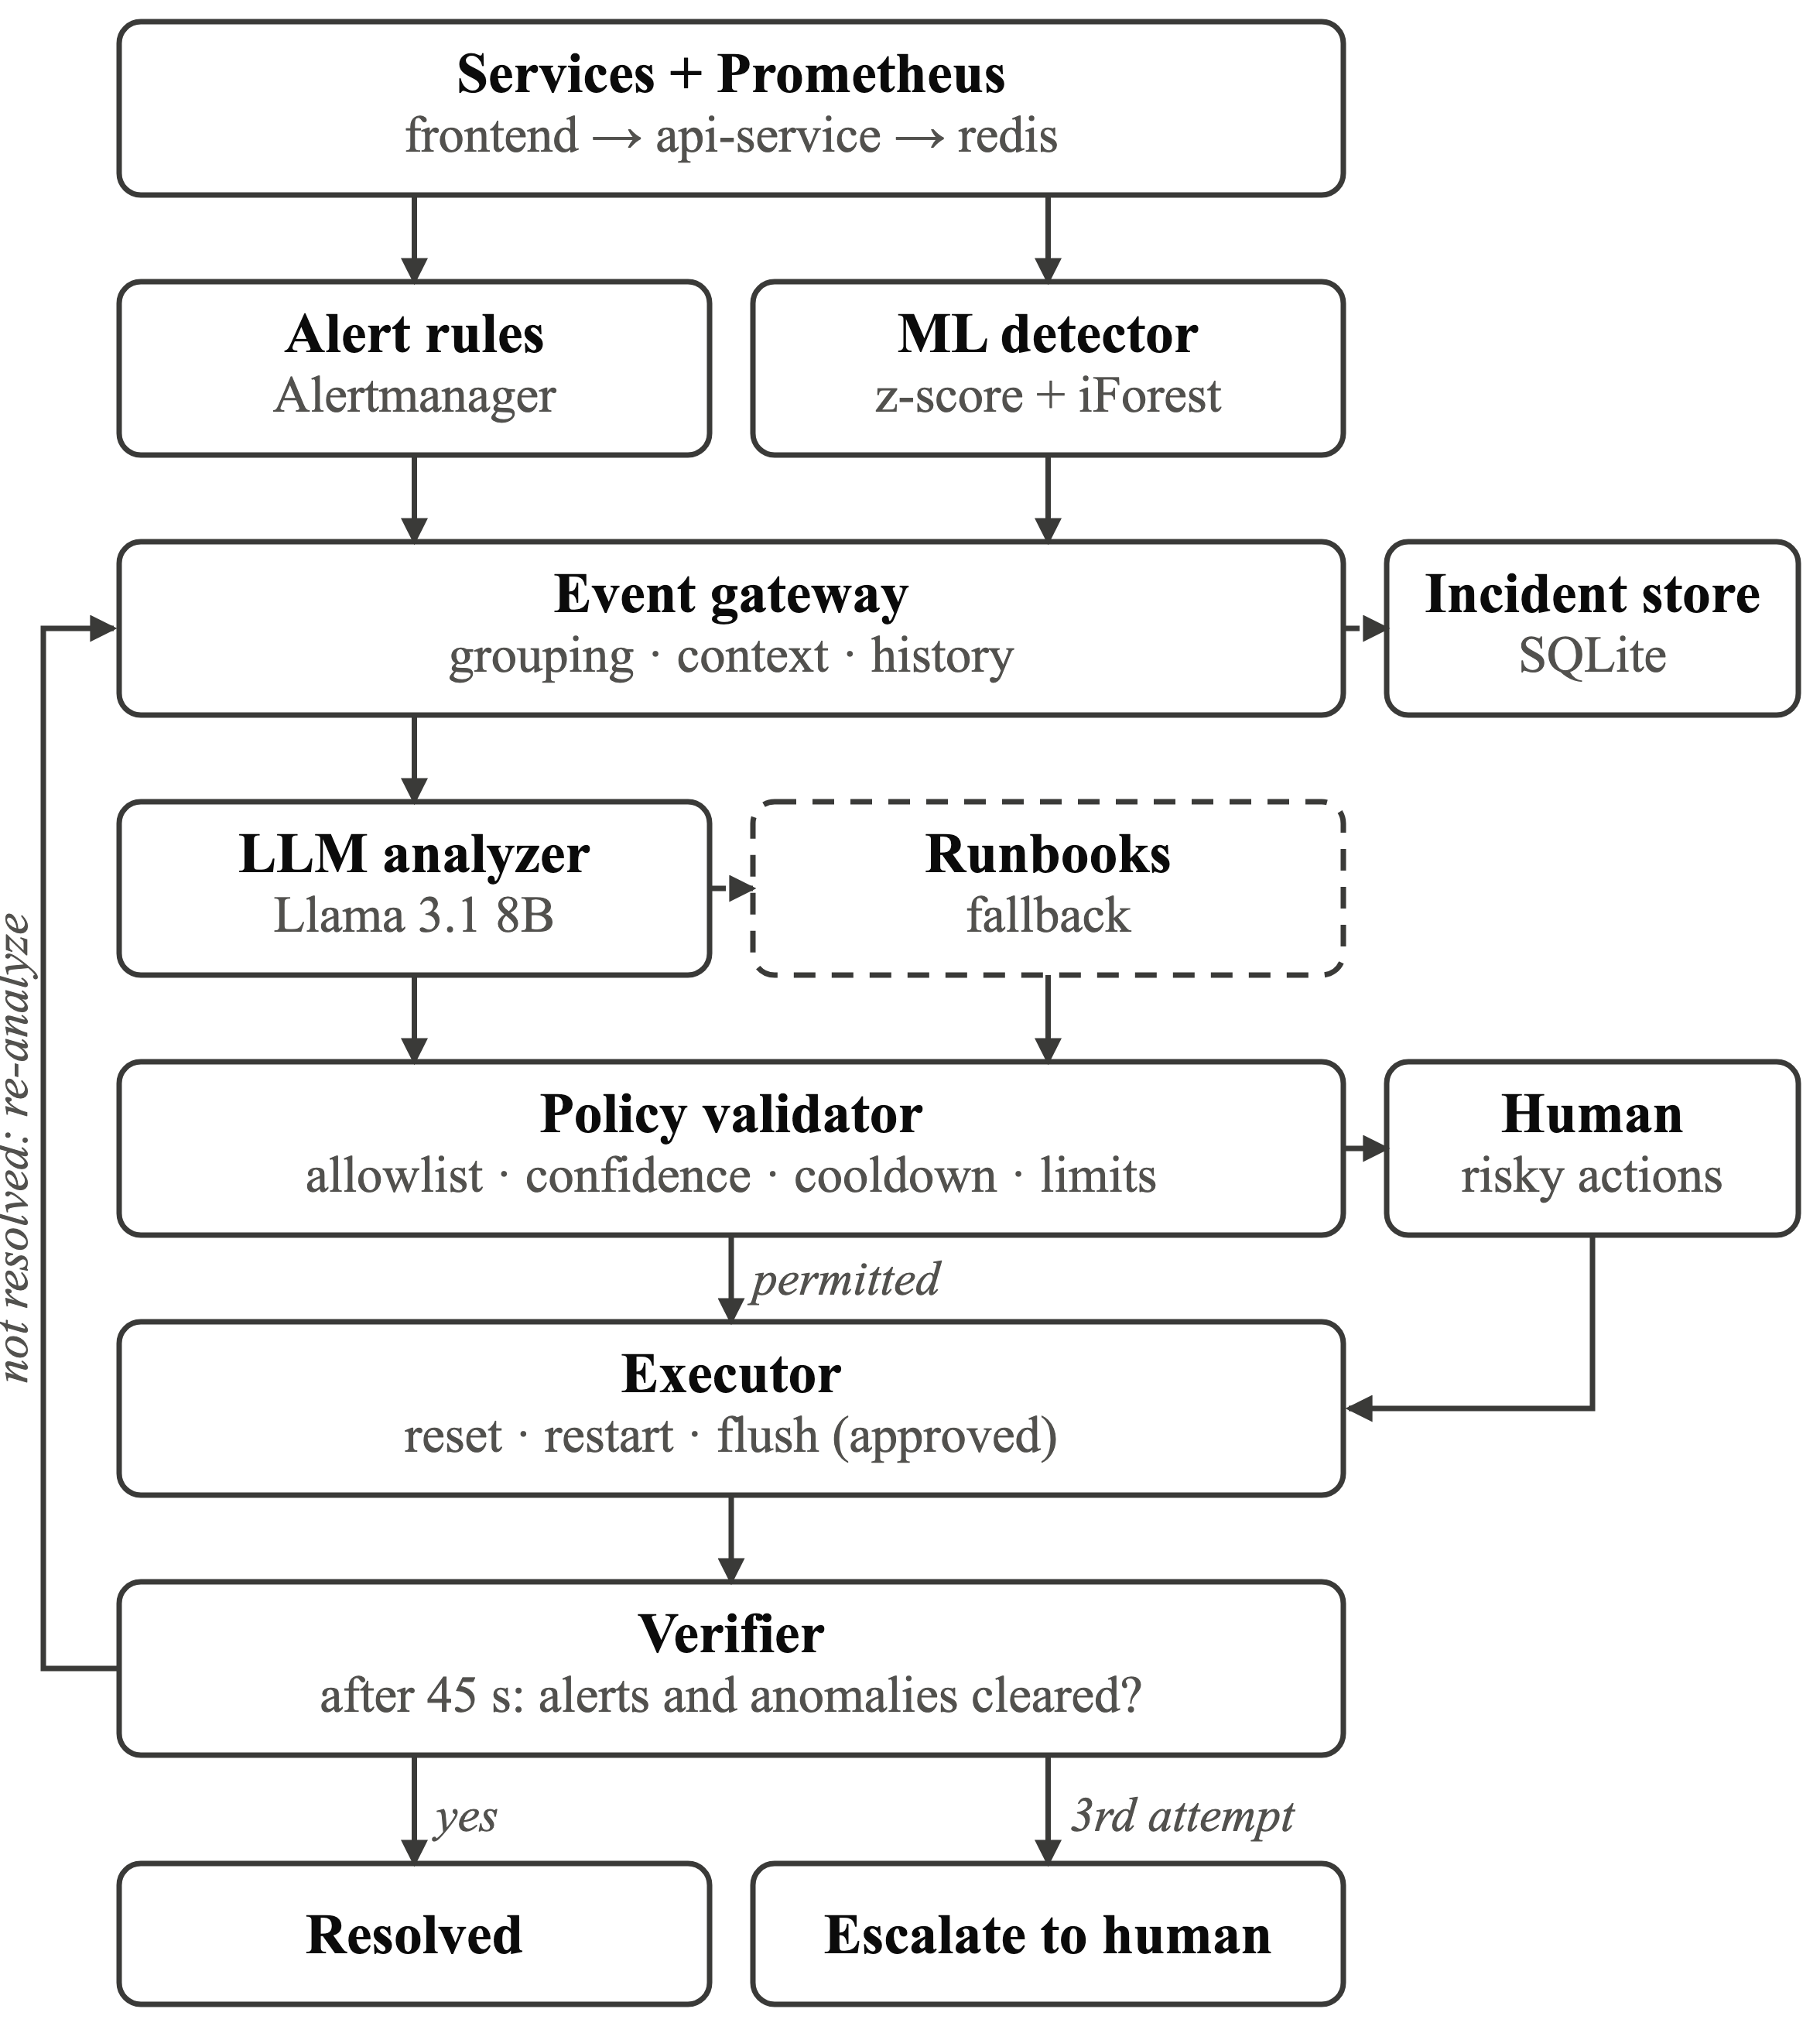
\includegraphics[width=\columnwidth]{fig1_architecture.png}
\caption{The architecture of the proposed system.}
\end{figure}

\subsection{Monitored Application and Detection}

The target will be a three-layer web application, where the frontend service invokes api-service that reads and increments a counter in Redis. The two Python services export request counts, latency histograms and an upstream-latency histogram; container CPU and memory metrics come from cAdvisor, and Prometheus \cite{b11} scrapes all targets every 5 s. Prometheus alert rules for high CPU, memory, latency, error rate and service unavailability use 30 s windows with a 20 s hold. A per-service anomaly detector, using robust z-scores \cite{b12} and an Isolation Forest \cite{b13} trained on fault-free traffic, adds early signals for faults that grow slowly or stay below the alert thresholds. Each service also exposes a fault-injection endpoint for the evaluation; its fault-state gauges are removed from every input of the system and used only for scoring.

\subsection{Event Gateway}

Alerts come from Alertmanager via a webhook and anomalies come from the detector. Signals received during 60 seconds from the services of the same call chain will be grouped into one incident, thus Redis failure and corresponding alerts from the API and frontend will be analyzed together. After a settle period of 10 s, the gateway builds the incident context: for each service the current values and ten-minute trends of CPU, memory, latency, error rate and upstream latency, the container status, the topology and the actions attempted so far. The incident is broadcast over a WebSocket and stored in SQLite.

\subsection{Analyzer}

Incidents will be converted by the analyzer to response plans consisting of: root cause service, incident type, severity, evidence, confidence level, recommended and alternative action with explanations. It prompts Llama 3.1 8B \cite{b14}, served locally by Ollama at temperature 0, with a system prompt, few-shot examples and the incident, and constrains the answer with a JSON schema. This answer is strictly type-checked, and the inclusion of confidence expressed as text or Boolean will be disregarded. In case there is an unavailability in reaching the model, a timeout, or an error in giving output with confidence less than 0.7, the analyzer will use deterministic YAML runbooks which describe a set of alert/anomaly to recommendation mappings. The analyzer can make only recommendations and has no access to the containers.

\subsection{Responder and Verifier}

The responder is the only part of the system that performs an action. In each plan, the responder verifies that the incident is still active, sends the plan for verification by the policy validator, invokes the permitted action via either the reset endpoint of the service or the Docker API, and after 45 seconds verifies that all alerts are resolved and that there is no active anomaly. If the incident remains active, then the responder requests the gateway to analyze the incident again together with the number of attempts made so far and the actions that have been tried before; this will be done for three times before escalation to a human.

\section{Safety Design}

The results of the analyzer will be considered untrusted input; any client can send a plan to the gateway, and the responder does not assume that the input adheres to the analyzer's schema. The policy validator will apply the validation rules specified in Table I to the recommended and fallback actions, respectively, taking the first one to succeed, else escalating the event. An action is considered to be unsafe if it is not on the allowlist, targets a component not permitted for it, or runs without a required approval.

\begin{table}[!t]
\caption{Policy Checks Applied to Every Plan}
\centering
\footnotesize
\renewcommand{\arraystretch}{1.15}
\setlength{\tabcolsep}{3pt}
\begin{tabular}{|>{\raggedright\arraybackslash}p{\dimexpr0.192\columnwidth-2\tabcolsep\relax}|>{\centering\arraybackslash}p{\dimexpr0.545\columnwidth-2\tabcolsep\relax}|>{\centering\arraybackslash}p{\dimexpr0.232\columnwidth-2\tabcolsep\relax}|}
\hline
\textbf{Check} & \textbf{Rule} & \textbf{On failure} \\ \hline
Allowlist & reset, restart, flush cache, update resources, escalate & fallback/escalate \\ \hline
Target & allowed service (no reset on Redis) & fallback/escalate \\ \hline
Confidence & a number in [0, 1] and at least 0.7 & human approval \\ \hline
Risk & flush cache, update resources & human approval \\ \hline
Cooldown & same action and target not within 300 s & fallback/escalate \\ \hline
Action limit & at most 3 executed actions per incident & escalate \\ \hline
Attempts & at most 3 analyze, act and verify cycles & escalate \\ \hline
\end{tabular}
\end{table}

This results in three tiers of autonomy: safe actions run automatically, dangerous or uncertain actions go to the approval queue, and the rest of the actions are forwarded to a human operator along with incident context and the set of actions that were tried. The executor implements only allowlisted actions, thus ensuring that there is no way to execute anything derived from a model sentence to a shell command. A pre-check prevents actions based on incidents that disappeared during planning, while the cooldown helps in stopping the loop if there is a recurring failure.

We constructed an adversarial set of 29 plans that will get through the real responder, using the recording executor: created new types of actions, shell commands as action parameters, targets external to the application, incorrect type of parameters (lists, null, boolean), missing confidence level, infinite or NaN, confidence levels out of bound, additional command fields, a valid action in the cooldown with a malicious fallback action, and reaching the maximum number of actions permitted. Five of those plans pass the analyzer's schema test, so only the responder's checks stop them. Building the suite revealed four input-handling bugs in the responder and the gateway, which were subsequently corrected; such bugs included the passing of the threshold test of the NaN confidence level since NaN \textless{} 0.7 is false and the interpreting of the Boolean value true as confidence 1.0. After correcting those bugs, all 29 plans conform to their specifications: the control plan is executed while all the adversary plans are blocked, stripped down or forwarded to a human.

\section{Evaluation Setup}

\subsection{Testbed and Fault Scenarios}

All experiments were performed on one laptop (Apple M4, 10 cores, 16 GB) with Docker Desktop; the LLM runs on the host. A Locust load generator sends about five requests per second. A fault injector starts each fault, logs its start and planned end, and polls the target until the fault is gone. A run counts as remediated if the fault is gone before its planned end, which only happens if the system fixed it. The scenarios are listed in Table II.

\begin{table}[!t]
\caption{Fault Scenarios: Known (1--9), Extra (10--14) and Unknown (15--19)}
\centering
\footnotesize
\renewcommand{\arraystretch}{1.15}
\setlength{\tabcolsep}{3pt}
\begin{tabular}{|>{\raggedright\arraybackslash}p{\dimexpr0.074\columnwidth-2\tabcolsep\relax}|>{\centering\arraybackslash}p{\dimexpr0.411\columnwidth-2\tabcolsep\relax}|>{\centering\arraybackslash}p{\dimexpr0.074\columnwidth-2\tabcolsep\relax}|>{\centering\arraybackslash}p{\dimexpr0.411\columnwidth-2\tabcolsep\relax}|}
\hline
\textbf{\#} & \textbf{Fault (expected action)} & \textbf{\#} & \textbf{Fault (expected action)} \\ \hline
1 & CPU load, frontend (reset or restart) & 10 & Corrupted cache value (flush, approval) \\ \hline
2 & CPU load, API (reset or restart) & 11 & Slow Redis writes (restart Redis) \\ \hline
3 & Memory 420 MB, API (restart) & 12 & Latency 0.6 s, API (reset) \\ \hline
4 & Latency 5 s, API (reset) & 13 & 5\% of requests fail, API (reset) \\ \hline
5 & All requests fail, API (reset) & 14 & Latency that returns after every fix (escalate) \\ \hline
6 & Redis stopped (restart Redis) & 15 & Latency 0.6 s, frontend (reset or restart) \\ \hline
7 & Frontend stopped (restart) & 16 & 5\% of requests fail, frontend (reset or restart) \\ \hline
8 & Memory leak, 440 MB over 240 s (restart) & 18 & CPU on frontend and errors on API (reset both) \\ \hline
9 & CPU and latency, API (reset) & 19 & Redis filled with 150 MB of keys (flush, approval) \\ \hline
\end{tabular}
\end{table}

Scenarios 1 to 9 form the core set of known faults, the ones the runbooks were written for, lasting 180 s (300 s for the leak). Scenarios 10 to 14 form an extra set of misleading, below-threshold and recurring faults lasting 300 s (480 s for scenario 14). Scenarios 15, 16, 18 and 19 form a third, unknown set of faults for which no runbook rule was written, lasting 300 s: subtle faults on the frontend, two faults at once, and a Redis memory fault. Existing rules still match 18 and 19, but the memory rule's restart cannot fix 19. We added this set after the first two had been evaluated and ran it on the unchanged system.

\subsection{Systems Compared}

\textit{B1}: alert rules and runbooks, without the LLM or the anomaly detector. \textit{B2}: alert rules and the LLM with runbook fallback, without the detector. B1 and B2 receive identical signals, so their difference isolates the analysis step. \textit{S}: the full system. \textit{SF}: the full system with the LLM unreachable, so that its runbooks act on the detector's incidents; it was run on scenarios 3, 4, 6 and 8 and on the unknown set. S and SF differ only in the analysis step, while SF and B1 differ only in the detector. The responder and the policies are identical across all variants.

\subsection{Protocol and Metrics}

Each round runs every scenario once per system in a shuffled order fixed by a seed, with rounds interleaved across systems and 300 s between consecutive runs, so the cooldown never carries over. The core set ran for 20 rounds (180 runs per system), the extra set for 10 rounds (190 runs) and the unknown set for 10 rounds on all four variants (160 runs); a run the laptop slept through was voided and repeated. We report the root-cause accuracy of the first plan; the correctness of the executed action against the expected action; unsafe actions; collateral actions, permitted actions on a service that was not the cause; the auto-resolution rate; the mean time to recover (MTTR, from fault start to fault gone, for remediated runs); the share of runs needing a second attempt; the escalation rate; and the LLM cost as plan latency and tokens per incident.

\section{Results}

\subsection{Safety (RQ1)}

In none of the 890 runs of the four variants was an unsafe action executed, and no incident was opened without an injected fault. Safety was not free: on the misleading faults of the extra set the variants executed 43, 35 and 36 collateral actions (B1, B2, S), resets and restarts of a healthy service that the policy permits, and S executed 8 more on the unknown set; the cooldown and the action limit capped these at three per incident. As no plans involved destructive acts in the live runs, the process of approval was carried out through the adversarial approach alone.

To see how the policy behaved in practice, we counted its decisions in the 562 incidents recorded by the incident store (core rounds 5 to 20, extra rounds 2 to 10). The allow list, target, and confidence tests never needed to block any live plan since all recommendations mentioned allowed actions, targets, and valid confidences; therefore, the tests' evidence comes from the adversarial suite. The guard intervened through the cooldown: on the extra set, the LLM variants recommended 46 (B2) and 45 (S) times to repeat a reset or restart that had just failed, each time the cooldown blocked it, and the responder ran the fallback action or escalated. The runbooks never did this because their plans for unmatched incidents escalate directly.

\subsection{Known Faults: LLM Versus Runbooks (RQ2)}

In the main scenarios, shown in Table III, all versions identified all faults. In all cases, B1 and B2 determined the actual cause, although the action taken was 100\% correct for B1 and 92.2\% correct for B2. All of B2's wrong actions were on scenario 5 (6/20 correct), where the LLM identified the correct service but restarted it rather than resetting its fault; the restart also cleared the fault, so the mistake cost time rather than safety.

\begin{table}[!b]
\caption{Results on the Core Scenarios (180 Runs per Variant)}
\centering
\footnotesize
\renewcommand{\arraystretch}{1.15}
\setlength{\tabcolsep}{3pt}
\begin{tabular}{|>{\raggedright\arraybackslash}p{\dimexpr0.385\columnwidth-2\tabcolsep\relax}|>{\centering\arraybackslash}p{\dimexpr0.196\columnwidth-2\tabcolsep\relax}|>{\centering\arraybackslash}p{\dimexpr0.196\columnwidth-2\tabcolsep\relax}|>{\centering\arraybackslash}p{\dimexpr0.192\columnwidth-2\tabcolsep\relax}|}
\hline
\textbf{Metric} & \textbf{B1} & \textbf{B2} & \textbf{S} \\ \hline
Detected & 100\% & 100\% & 100\% \\ \hline
Root cause correct & 100\% & 100\% & 97.2\% \\ \hline
Executed action correct & 100\% & 92.2\% & 93.9\% \\ \hline
Unsafe actions executed & 0 & 0 & 0 \\ \hline
Auto-resolved & 100\% & 100\% & 99.4\% \\ \hline
MTTR mean (s) & 75.3 & 104.9 & 74.1 \\ \hline
MTTR without scenario 8 (s) & 53.0 & 82.3 & 70.8 \\ \hline
MTTR 90th percentile (s) & 249.8 & 281.5 & 98.9 \\ \hline
MTTR worst run (s) & 261.4 & 290.4 & 139.7 \\ \hline
Runs needing a 2nd attempt & 0 & 0 & 7 \\ \hline
Escalated & 0\% & 0\% & 0.6\% \\ \hline
\end{tabular}
\end{table}

The LLM was also slower: a runbook plan takes milliseconds to produce, while the LLM needed 28.4 s per plan on this laptop. Fig.~2 illustrates the impact on recovery: it plots the mean time to recover of B1, B2 and S in each of the nine core scenarios, and the B2 bar is higher than the B1 bar in all of them. Excluding scenario 8, mean MTTR was 53.0 s for B1 and 82.3 s for B2, about 29 s more per incident. The difference is systematic: in each of the nine core scenarios every B2 run took longer than every B1 run (Mann-Whitney U = 0, p \textless{} 10$^{-7}$ per scenario), with a median shift of 26 to 36 s (Hodges-Lehmann; 30 s over scenarios 1 to 7 and 9). On the faults the runbooks were written for, the runbooks were therefore both more accurate and faster.

\begin{figure}[!b]
\centering
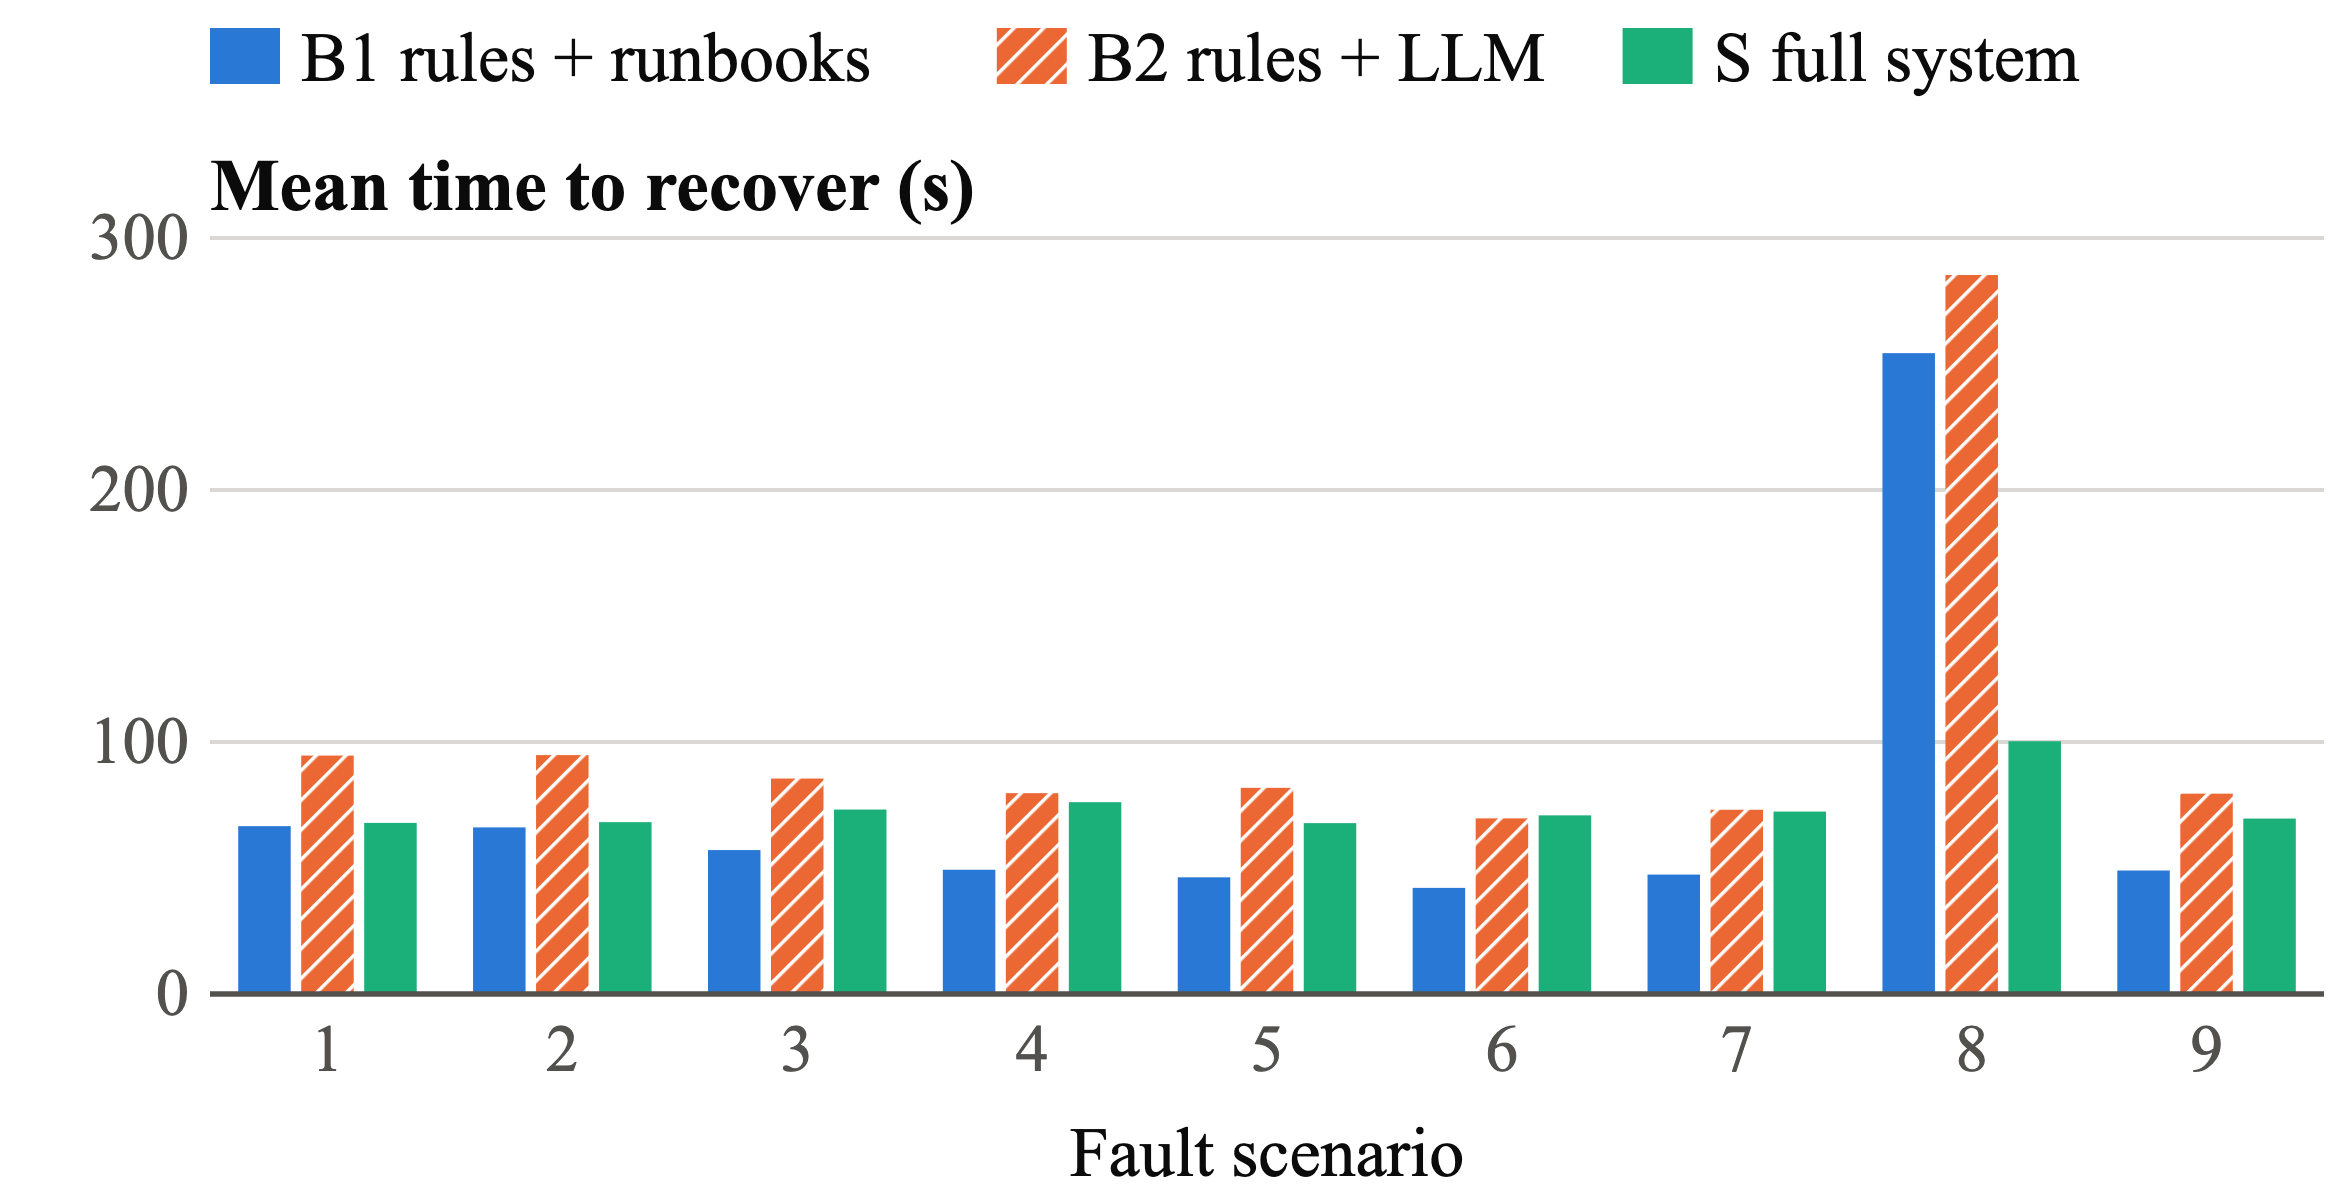
\includegraphics[width=\columnwidth]{fig2_mttr.png}
\caption{Mean time to recover per core scenario (20 runs per bar).}
\end{figure}

The minimum average MTTR (74.1 s) obtained by S is due to the performance of scenario 8, which shows a gradual memory leak, which is detected by S's anomaly detector much earlier than the memory alarm triggers (100 s versus 285 s of B2). This benefit is based on the detection process rather than analysis; without scenario 8, S (70.8 s) ranks between B1 and B2. S was also more consistent in its recovery times: 90\% of its trials recovered in 98.9 seconds with a maximum of 139.7 s, versus 249.8 s and 261.4 s of B1 since no fault in S relied on a slow alarm before taking action.

\subsection{Unknown Faults (RQ3)}

The results of the unknown set are given in Table IV. The subtle frontend faults (15 and 16) stayed under the warning limits, so that neither B1 nor B2 reacted to them. The anomaly detector found the latency fault (15) in every S and SF run. With the LLM unavailable, SF had no runbook rule for an anomaly-only latency incident and escalated all ten runs; S resolved 8 of 10, 6 after a correct first reset of the frontend in 58 to 70 s, and 2 after the verify loop corrected a first plan that blamed the api-service (208 and 212 s); the other 2 were escalated. The detector found this fault and the LLM fixed it; neither did so alone. The 5 percent error fault (16) is intermittent and was detected in only 4 S runs and 1 SF run, and it was never resolved.

\begin{table}[!t]
\caption{Unknown Faults: Detected / Resolved / Escalated Runs of 10}
\centering
\footnotesize
\renewcommand{\arraystretch}{1.15}
\setlength{\tabcolsep}{3pt}
\begin{tabular}{|>{\raggedright\arraybackslash}p{\dimexpr0.313\columnwidth-2\tabcolsep\relax}|>{\centering\arraybackslash}p{\dimexpr0.164\columnwidth-2\tabcolsep\relax}|>{\centering\arraybackslash}p{\dimexpr0.164\columnwidth-2\tabcolsep\relax}|>{\centering\arraybackslash}p{\dimexpr0.164\columnwidth-2\tabcolsep\relax}|>{\centering\arraybackslash}p{\dimexpr0.164\columnwidth-2\tabcolsep\relax}|}
\hline
\textbf{Scenario} & \textbf{B1} & \textbf{B2} & \textbf{S} & \textbf{SF} \\ \hline
15 Frontend latency & 0 / 0 / 0 & 0 / 0 / 0 & 10 / 8 / 2 & 10 / 0 / 10 \\ \hline
16 Frontend errors & 0 / 0 / 0 & 0 / 0 / 0 & 4 / 0 / 2 & 1 / 0 / 1 \\ \hline
18 Two faults & 10 / 10 / 0 & 10 / 10 / 0 & 10 / 10 / 0 & 10 / 6 / 4 \\ \hline
19 Redis memory & 10 / 0 / 7 & 10 / 0 / 8 & 10 / 0 / 10 & 10 / 0 / 10 \\ \hline
Resolved (of 40) & 10 & 10 & 18 & 6 \\ \hline
Verified, fault stayed & 3 & 2 & 0 & 0 \\ \hline
\end{tabular}
\end{table}

The combined fault (18) fires the usual error alert, and B1, B2 and S resolved it in every run, one service per attempt (S needed a third attempt once); B1 was fastest (91 s against 143 s for S). SF resolved 6, escalating when its incident opened on the anomaly before the alert. In the Redis memory fault (19), every variant named Redis and restarted it, but Redis reloaded the keys from disk, so the fault remained; no plan, from the LLM or a runbook, suggested flushing the cache. Anomaly persisted and the escalation occurred on all runs by S and SF. The verifiers from B1 and B2 took the restart without detector due to the memory alarm clearing for some period of time, and then the memory alarm raised another incident. Over the 40 runs, S resolved 18, B1 and B2 10 each, and SF 6.

\subsection{Wrong Diagnoses and the Verify Loop (RQ4)}

In 5 out of 180 first plans made by S, the incorrect root cause was chosen. The incidents initiated by S often start with a premature anomaly; hence, the evidence at this stage is insufficient -- this is the cost of acting fast. The verify loop was able to solve 4 of these problems. For instance, in scenario 6, the first plan was wrong because it accused api-service of causing the failure of Redis, while in scenario 4, the first plan incorrectly blamed the frontend for the increased latency of the API. The problem remained unfixed, the verifier put the incident back into the queue with the failed action included into its history, and the second plan operated the right service. In those cases, the recovery time was 124--140 s compared to 70 s achieved otherwise, but no damage was done. In one run, however, an early runbook plan escalates the incident mere seconds before the correct LLM plan comes up, and the responder then ignored the LLM plan. Seven S runs had to retry (the other three after a correct fix that the verifier judged unresolved while an anomaly faded); none of B1 or B2 did.

\subsection{Misleading and Recurring Faults (RQ4)}

The results for the extra set are summarized in Table V. In the two misleading Redis faults (10 and 11), Redis keeps running while the api-service shows the errors or latency. All variants, the LLM included, blamed the api-service (a single S run blamed the frontend); no plan proposed flushing the cache or restarting Redis. The cooldown, fallback and action limit kept the response bounded, and all 60 of these runs were escalated to a human with the actions already attempted. The recurring fault (14) was escalated in all 30 runs after the reset and the restart failed, as intended. The below-threshold faults (12 and 13) did not trigger alerts, so B1 and B2 never intervened; through its anomaly detector, S detected scenario 12 in 10/10 and scenario 13 in 5/10 runs, and resolved scenario 12 in 10 of 10 runs. In scenario 13 the intermittent anomaly was older than the responder's freshness window when four LLM plans arrived, so the pre-check skipped them as already cleared; the fifth detected run was escalated by a runbook plan.

\begin{table}[!t]
\caption{Extra Scenarios: Detected / Resolved / Escalated Runs of 10}
\centering
\footnotesize
\renewcommand{\arraystretch}{1.15}
\setlength{\tabcolsep}{3pt}
\begin{tabular}{|>{\raggedright\arraybackslash}p{\dimexpr0.369\columnwidth-2\tabcolsep\relax}|>{\centering\arraybackslash}p{\dimexpr0.200\columnwidth-2\tabcolsep\relax}|>{\centering\arraybackslash}p{\dimexpr0.200\columnwidth-2\tabcolsep\relax}|>{\centering\arraybackslash}p{\dimexpr0.200\columnwidth-2\tabcolsep\relax}|}
\hline
\textbf{Scenario} & \textbf{B1} & \textbf{B2} & \textbf{S} \\ \hline
10 Corrupted cache & 10 / 0 / 10 & 10 / 0 / 10 & 10 / 0 / 10 \\ \hline
11 Slow Redis & 10 / 0 / 10 & 10 / 0 / 10 & 10 / 0 / 10 \\ \hline
12 Latency 0.6 s & 0 / 0 / 0 & 0 / 0 / 0 & 10 / 10 / 0 \\ \hline
13 5\% errors & 0 / 0 / 0 & 0 / 0 / 0 & 5 / 0 / 1 \\ \hline
14 Recurring latency & 10 / 0 / 10 & 10 / 0 / 10 & 10 / 0 / 10 \\ \hline
\end{tabular}
\end{table}

\subsection{LLM Unavailable and Cost (RQ4)}

With the LLM unreachable, SF fell back to the runbooks and resolved 34 of 40 known-fault runs, the memory, Redis and leak faults in every run and faster than S, since no LLM call was made. In 6 of 10 latency runs (scenario 4), the incident opened on an anomaly before the latency alert fired, no runbook matched an anomaly-only latency incident, and the fallback plan escalated it early; the same gap caused its escalations in scenarios 15 and 18 of the unknown set. An incident in S used 1.7 LLM calls on average, with about 4284 prompt and 261 completion tokens on the core set; with a local model this costs time, not money, about 27.0 s per plan.

\section{Discussion and Limitations}

\textit{What the guard provides.} The mistakes that the LLM made turned out to be the ones that the guard could catch: the weak action in case of a known fault, the symptom service that reported the wrong fault, and the repeated failed action despite multiple reanalyses (45 times in S), even though it was already mentioned in the incident history. In all cases, the result was constrained by the policy layer and verify loop, and not the model itself. The safety was thus ensured regardless of the quality of the model, which is important since an operator cannot verify all model recommendations in advance.

\textit{Each has its distinct function.} For the known faults, the LLM brought about latency and no accuracy, while for the misleading faults, the LLM performed similarly to the runbooks. For the unknown faults, the LLM was the only step of analysis that solved the latency fault, since the detector had already discovered the problem, and the detector without the LLM could only escalate, while the LLM without the detector would never encounter the fault at all. The detector also made sure the verifier did not accept a restart that would not work. Thus, a deployment strategy should match the known patterns with the runbooks, invoke the LLM when no runbook applies, and employ the same guard for both. However, the LLM is not a cure-all -- for the Redis memory fault, the LLM proposed the same ineffective restart as the runbook.

\textit{Validity:} The errors are induced via the endpoint, and hence, the reset operation represents a rollback or the use of feature flagging in production. The testbed consists of a single laptop running three services, the synthetic load, and an 8-billion parameter model, and using a bigger model could be useful in finding out the misleading faults. The unknown set has four cases which were generated by the authors after the first evaluation, and hence, it is representative of the areas where the LLM could be helpful rather than its frequency. There is a need for a manual baseline where an engineer takes care of the errors to compare the amount of time saved.

\section{Conclusion}

We proposed a closed-loop system of incident response in which the decision on what to run is taken at the policy layer, and not by the LLM itself. No unsafe actions were performed in 890 runs on real containers or in 29 adversarial plans; the verify loop fixed wrong initial diagnosis, and confusing or recurrent failures were escalated after a limited number of tries. The runbooks were better than the LLM in the accuracy of selected actions and in the speed on the known faults; on unknown faults, the combination of the detector and the LLM was able to fix 18 runs of 40 against 10 by the runbooks.

\begin{thebibliography}{00}
\bibitem{b1} B. Beyer, C. Jones, J. Petoff, and N. R. Murphy, Eds., \textit{Site Reliability Engineering: How Google Runs Production Systems}. Sebastopol, CA, USA: O'Reilly Media, 2016.
\bibitem{b2} Y. Dang, Q. Lin, and P. Huang, ``AIOps: Real-world challenges and research innovations,'' in \textit{Proc. IEEE/ACM Int. Conf. Software Engineering: Companion (ICSE-Companion)}, 2019.
\bibitem{b3} T. Ahmed, S. Ghosh, C. Bansal, T. Zimmermann, X. Zhang, and S. Rajmohan, ``Recommending root-cause and mitigation steps for cloud incidents using large language models,'' in \textit{Proc. IEEE/ACM Int. Conf. Software Engineering (ICSE)}, 2023.
\bibitem{b4} Y. Chen et al., ``Automatic root cause analysis via large language models for cloud incidents,'' in \textit{Proc. European Conf. Computer Systems (EuroSys)}, 2024.
\bibitem{b5} k8sgpt-ai, ``k8sgpt: Giving Kubernetes superpowers to everyone,'' GitHub repository. Accessed: Oct. 26, 2026. [Online]. Available: \url{https://github.com/k8sgpt-ai/k8sgpt}
\bibitem{b6} Robusta, ``HolmesGPT,'' GitHub repository. Accessed: Oct. 26, 2026. [Online]. Available: \url{https://github.com/robusta-dev/holmesgpt}
\bibitem{b7} L. Wu, J. Tordsson, E. Elmroth, and O. Kao, ``MicroRCA: Root cause localization of performance issues in microservices,'' in \textit{Proc. IEEE/IFIP Network Operations and Management Symp. (NOMS)}, 2020.
\bibitem{b8} Y. Chen et al., ``AIOpsLab: A holistic framework to evaluate AI agents for enabling autonomous clouds,'' 2025, arXiv:2501.06706. [Online]. Available: \url{https://arxiv.org/abs/2501.06706}
\bibitem{b9} T. Rebedea, R. Dinu, M. Sreedhar, C. Parisien, and J. Cohen, ``NeMo Guardrails: A toolkit for controllable and safe LLM applications with programmable rails,'' in \textit{Proc. Conf. Empirical Methods in Natural Language Processing: System Demonstrations (EMNLP)}, 2023.
\bibitem{b10} A. Basiri et al., ``Chaos engineering,'' \textit{IEEE Software}, vol. 33, no. 3, pp. 35--41, 2016.
\bibitem{b11} Prometheus Authors, ``Prometheus documentation.'' Accessed: Oct. 26, 2026. [Online]. Available: \url{https://prometheus.io/docs/}
\bibitem{b12} P. J. Rousseeuw and C. Croux, ``Alternatives to the median absolute deviation,'' \textit{J. American Statistical Association}, vol. 88, no. 424, pp. 1273--1283, 1993.
\bibitem{b13} F. T. Liu, K. M. Ting, and Z.-H. Zhou, ``Isolation forest,'' in \textit{Proc. IEEE Int. Conf. Data Mining (ICDM)}, 2008, pp. 413--422.
\bibitem{b14} A. Grattafiori et al., ``The Llama 3 herd of models,'' 2024, arXiv:2407.21783. [Online]. Available: \url{https://arxiv.org/abs/2407.21783}
\end{thebibliography}
\end{document}
